\chapter{Spark自动缓存模块设计与实现}\label{chap:auto-cache}

本章首先对Spark缓存管理机制进行了深入的分析,从而引出了自动缓存的需求。之后详细阐述了自动缓存模块的设计与实现,最后介绍了测试数据集SparkBench,并对自动缓存模块进行了一系列的测试。

\section{Spark相关模块现状分析}
Spark框架相对于Hadoop的核心改进是添加了缓存管理模块。通过将计算过程中的中间数据缓存在内存中可以极大的加速计算过程。尤其对于机器学习和图计算等迭代式计算有上百倍的加速效果。这是因为这种迭代式计算需要多次重复访问中间数据,就非常能体现Spark框架的优势。

\subsection{缓存模块底层原理}
Spark应用在执行过程中会将应用程序解析成DAG图,然后根据DAG的拓扑排序顺序执行DAG图中的每一个操作。一个RDD数据被计算得到之后,会存放在Execution Memory区域。如果没有立即被使用使用到就会从Execution Memory区域被删除。Spark框架给应用程序员提供了cache接口,cache接口会将RDD对象的STORAGE\_LEVEL字段标记为MEMORY\_ONLY。标记之后Spark框架并不会立即缓存数据,而是在RDD分区数据计算完成时查看STORAGE\_LEVEL标记。根据不同的标记将数据缓存到不同的位置,常见的标记有以下几种,MEMORY\_ONLY,DISK\_ONLY,MEMORY\_AND\_DISK。如果标记为MEMORY\_ONLY框架就会将数据缓存到内存之中,具体过程是将RDD的应用发送给BlockManager对象的MemoryStore模块。MemoryStore模块会保存RDD模块的引用。这样就能将RDD对象长时间保存在内存中。从缓存管理模块的逻辑视图角度来看cache接口调用是将RDD对象从Execution Memory区域移到了Storage Memory区域。如果STORAGE\_LEVEL标记为DISK\_ONLY。框架会将RDD对象的引用发送给BlockManager的DiskStore模块。DiskStore模块在HDFS或者其他文件系统上创建一个文件,将RDD对象写入文件之中。并且保存文件的路径。这就是缓存管理模块的核心过程。

当要使用到一个RDD数据时,框架会从BlockManager模块查看数据是否存在缓存数据。此时有两种情况,如果缓存数据存放在磁盘之中框架会将数据读取加载到内存的Execution Memory区域。如果是缓存在内存之中就可以直接进行计算。

在分析了缓存模块的核心原理之后还有一个重要的问题,就是缓存决策是如何实现的。目前Spark应用的缓存决策全都由编程人员在开发的过程中手动指定。这存在着几个问题。第一,编程人员可能会做出不正确的缓存决定,缓存了无用的数据,这会导致内存被浪费,降低了系统内存资源的使用效率。第二,编程人员可能没有缓存重要数据,导致在计算的过程中重复计算重要数据,对应用程序的执行时间造成巨大的影响。第三,这种编程模式对Spark应用编程人员提出了比较高的要求,编程人员必须熟悉Spark框架的核心原理,还要熟悉Spark提供的众多算子的底层实现,在此基础上还需要在编程的过程中选择合适的数据进行缓存,在Spark应用程序规模变大之后就会对编程人员造成比较大的负担。

\subsection{自适应执行框架原理}
同时还需要考虑Spark框架最新的动态执行新特性。Spark框架本身是在不断发展之中,Spark这类并行数据处理系统存在着一些问题,下面三个问题对性能影响比较突出:

\begin{enumerate}
    \item shuffle partition 个数,比如spark的shuffle partition个数默认值为200。可以通过参数配置,这个参数决定了reduce阶段任务的数量,对整个查询的性能有很大的影响。假设一个查询运行前申请E个Executor,每个Executor包含C个core(并发执行线程数),那么该作业在运行时可以并行执行的作业个数就为$E\times C$个,也可以说该作业的并发数为$E\times C$个。假设shuffle partition个数为P,处理map stage的任务数和原始数据的文件数量和大小有关,后续的每个reduce stage的任务数量都为P。由于Spark作业调度是抢占式的,$E\times C$个作业会抢占执行P个任务,直至所有任务完成,就会进入下一个stage。在这个过程中,任务执行时间会过长,导致整个stage执行时间变长,另一方面,$E\times C$个执行单元大部分都处于空闲状态,导致整体资源利用率急剧下降。所以shuffle partition个数的设置就对性能有着很大的影响,在实际运行场景下,作业执行之前很难设置shuffle partion个数。
    \item 最佳执行计划,Spark SQL会将应用程序翻译成逻辑计划,然后经历一系列的优化,最后确定一个物理执行计划。最终选择的物理执行计划对性能有很大的影响。如果选择最佳的执行计划是Spark SQL的Catalyst优化器的核心工作。Catalyst早期主要是基于规则的优化器(RBO,Rule Based Optimizer),在Spark2.2中加入了基于代价的优化(CBO, Cost Based Optimizer)。也有一些工作实现了根据历史记录的优化(HBO,History Based Optimizer)。这些优化器统一的特点是在作业执行之前完全确定物理执行计划,一旦确定之后就不再改变。然而实际作业往往在事先无法完全预料。如图\ref{fig:wrong-sort-join}所示。其中一张表的大小仅为600KB,然后Spark申城的物理执行计划依旧使用了sortMergeJoin。这种场景明显使用BroadcastJoin更加合理。
    \item 数据倾斜问题。数据倾斜是常见的导致SparkSQL性能变差的问题。数据倾斜是指某一个partition的数据量远远大于其他partition的数据。导致个别任务的运行时间远远大于其他任务,因此拖累了整个作业的运行时间。在实际作业中,数据倾斜问题很常见,这是因为join key对应的hash值分布不均匀。在极端情况下,hash结果分布非常不均匀,导致大量数据被分到同一个partition二导致严重数据倾斜。如图\ref{tab:data-qinxie}所示,大部分任务在两秒内就完成了,但是最慢的任务却花了4分钟,这就是因为发生了数据倾斜问题,他处理的数据是其他任务的数倍。最终虽然大部分很快就运行结束,因为数据倾斜问题,整个作业的执行时间也被极大地影响了。

\end{enumerate}

\begin{figure}
    \centering
    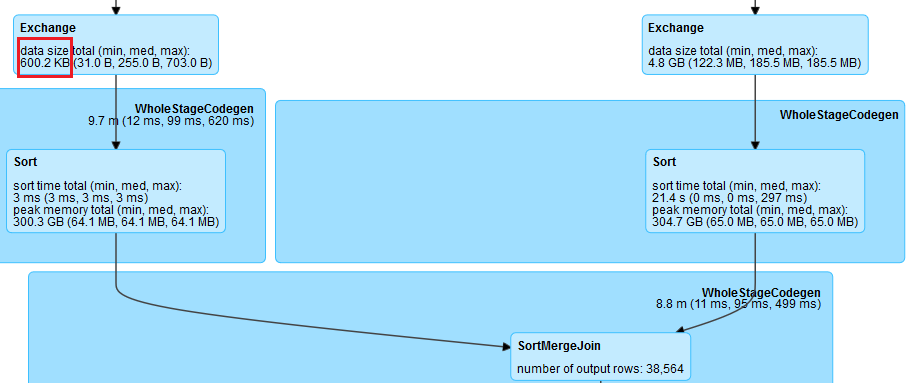
\includegraphics[width=0.99\textwidth]{Img/wrong-sort-join.png}
    \caption{不合理的物理执行计划}
    \label{fig:wrong-sort-join}
\end{figure}


\begin{table}
 \centering
 \small
 \caption{SparkBenck支持的负载}
 \label{tab:data-qinxie}
 \resizebox{\columnwidth}{!}{%
 \begin{tabular}{lccccccccl}
  \toprule
  Metric & Min & 25th percentile & Median & 75th percentile & Max \\
  \midrule
  Duration & 15ms & 2s  & 3s  & 5s & 4min \\
  Scheduler Delay & 0ms & 2ms & 2ms & 3ms & 1s \\
  Task Deserialization Time & 3ms & 5ms & 6ms & 7ms & 0.4s \\
  GC Time & 0ms & 0ms & 0.2s & 0.3s & 35s \\
  Result Serialization Time & 0ms & 0ms & 0ms & 0ms & 3ms \\
  Getting Result Time & 0ms & 0ms & 0ms & 0ms & 0ms \\
  Peak Execution Memory & 0B & 0B & 0B & 0B & 0B \\
  Shuffle Read Blocked Time & 0ms & 44ms & 0.2s & 0.6s & 31s \\
  Shuffle Read Size/Records & 0B/0 & 3.5MB/374415 & 4.0MB/747052 & 6.9MB/1783859 & 172.8MB/283732661 \\
  Shuffle Write Size/Records & 0B/0 & 109B/3 & 132B/4 & 158B/6 & 262B/13 \\
  Shuffle spill(memory) & 0B & 0B & 0B & 0B & 13.3GB \\
  Shuffle Write(disk) & 0B & 0B & 0B & 0B & 68.2MB \\
  \bottomrule
 \end{tabular}}
\end{table}

对于这些问题,Spark设计实现了一套自适应执行框架。自适应执行框架的思路是在执行计划中划分好stage,然后按照stage提交执行,在运行过程中收集当前stage的统计信息,通过运行时信息来优化下一个stage的物理执行计划,然后提交后续的stage。在运行过程中,Spark动态执行框架会根据运行情况动态设置下游Reducer个数、动态调整执行计划、动态处理数据倾斜问题。

\section{自动缓存模块}

\subsection{自动缓存模块设计}
通过上文对Spark相关模块的详细分析后,本文设计了一种改进的自动缓存模块。需要实现自动缓存的功能,就需要能够判断在整个作业计算过程中哪些数据会被重复使用,对于需要重复使用的RDD数据,应该将其缓存在缓存之中,这样在之后的计算过程中,Spark框架就可以直接使用已经缓存的数据进行计算,从而能够加速计算过程。

针对Spark底层实现原理来分析,Spark会将应用程序转化为一个DAG图,这里使用$G(V, E)$来表示DAG。DAG图中的节点$V$是RDD数据,DAG图中的边$E$为RDD数据之间的转化关系,分为transformation和action两种。根据action操作,Spark框架会将整个DAG切分成多个作业,这里用$J={j_1, j_2,...,j_m }$表示所有作业。对于每个作业$j_i$,Spark框架会根据宽依赖将作业分为多个stage。如果$RDD_i$通过操作转化为$RDD_j$,其中存在一条边$(i, j)\in E$,那么$RDD_i$就称为$RDD_j$的父节点。对于$RDD_v$来说,它的所有父节点记为$anc(v)$。它的所有后继节点记为$dsc(v)$。

根据对Spark底层DAG图结构进行分析之后发现需要得到应用对应的DAG图,只要得到了DAG图,然后对DAG图进行分析就可以得到重复使用的RDD数据,在DAG图中,对于$RDD_v$, $dsc(v)$的大小就是会被重复使用的次数。在程序运行之前是很难得到DAG图结构,所以可以使用少量输入数据运行整个应用程序,然后记录DAG图结构。之后使用全量输入数据再次运行整个程序,这样就可以在第二次执行过程中缓存需要重复使用的数据。

在上文介绍了Spark的动态执行功能。动态执行功能会在执行过程中根据stage的运行时数据优化调整接下来的物理执行计划,所以当Spark调整执行计划时,自动缓存模块也需要同步更新修改DAG图结构,这样就可以保持正确的DAG图结构。

\subsection{自动缓存模块实现}
Spark应用程序都会创建一个SparkContext,SparkContext对应了一个Spark应用程序的生命周期,SparkContext中包含着RDD根节点,DAGScheduler,TaskScheduler,SchedulerBackend, BlockManager。本文所做的工作大多是修改SparkContext内的各个组件完成的。

SparkContext对象创建之后会初始化各个组件,初始化完成之后就会开始执行用户代码。Spark应用一般从读取数据开始,SparkContext提供了许多接口从文件系统中读取数据,Spark框架会创建一个新的RDD对象,在RDD对象的data字段存储这指向实际数据的应用。RDD对象有一个指向父节点的引用dependency, 输入节点RDD有一个特点,就是它的dependency是指向sparkContext对象的。所以sparkContext相当于是整个DAG图的根节点。

为了得到整个DAG图的结构,需要使用小量数据运行整个应用程序,得到DAG图结构。这就需要修改输入RDD节点,之前说过RDD节点是只读的,这种特性是利用了Scale语言的特性,将data字段设置为不可变的value对象。所以需要将data改为可变数据variable。这样就可以替换输入数据为小规模数据。同时还需要将全局RDD的STORAGE\_LEVEL字段设置为MEMORY\_ONLY,这是为了得到一个正确的DAG图结构。在计算结束之后,就可以得到完整的DAG图。Spark应用在结束的时候会调用sparkContext.stop接口结束整个应用并释放所有资源,所以可以修改stop接口,将数据替换为全量数据,重新运行整个作业之后结束整个作业。完整的流程如图\ref{fig:auto-cache}所示。

\begin{figure}
    \centering
    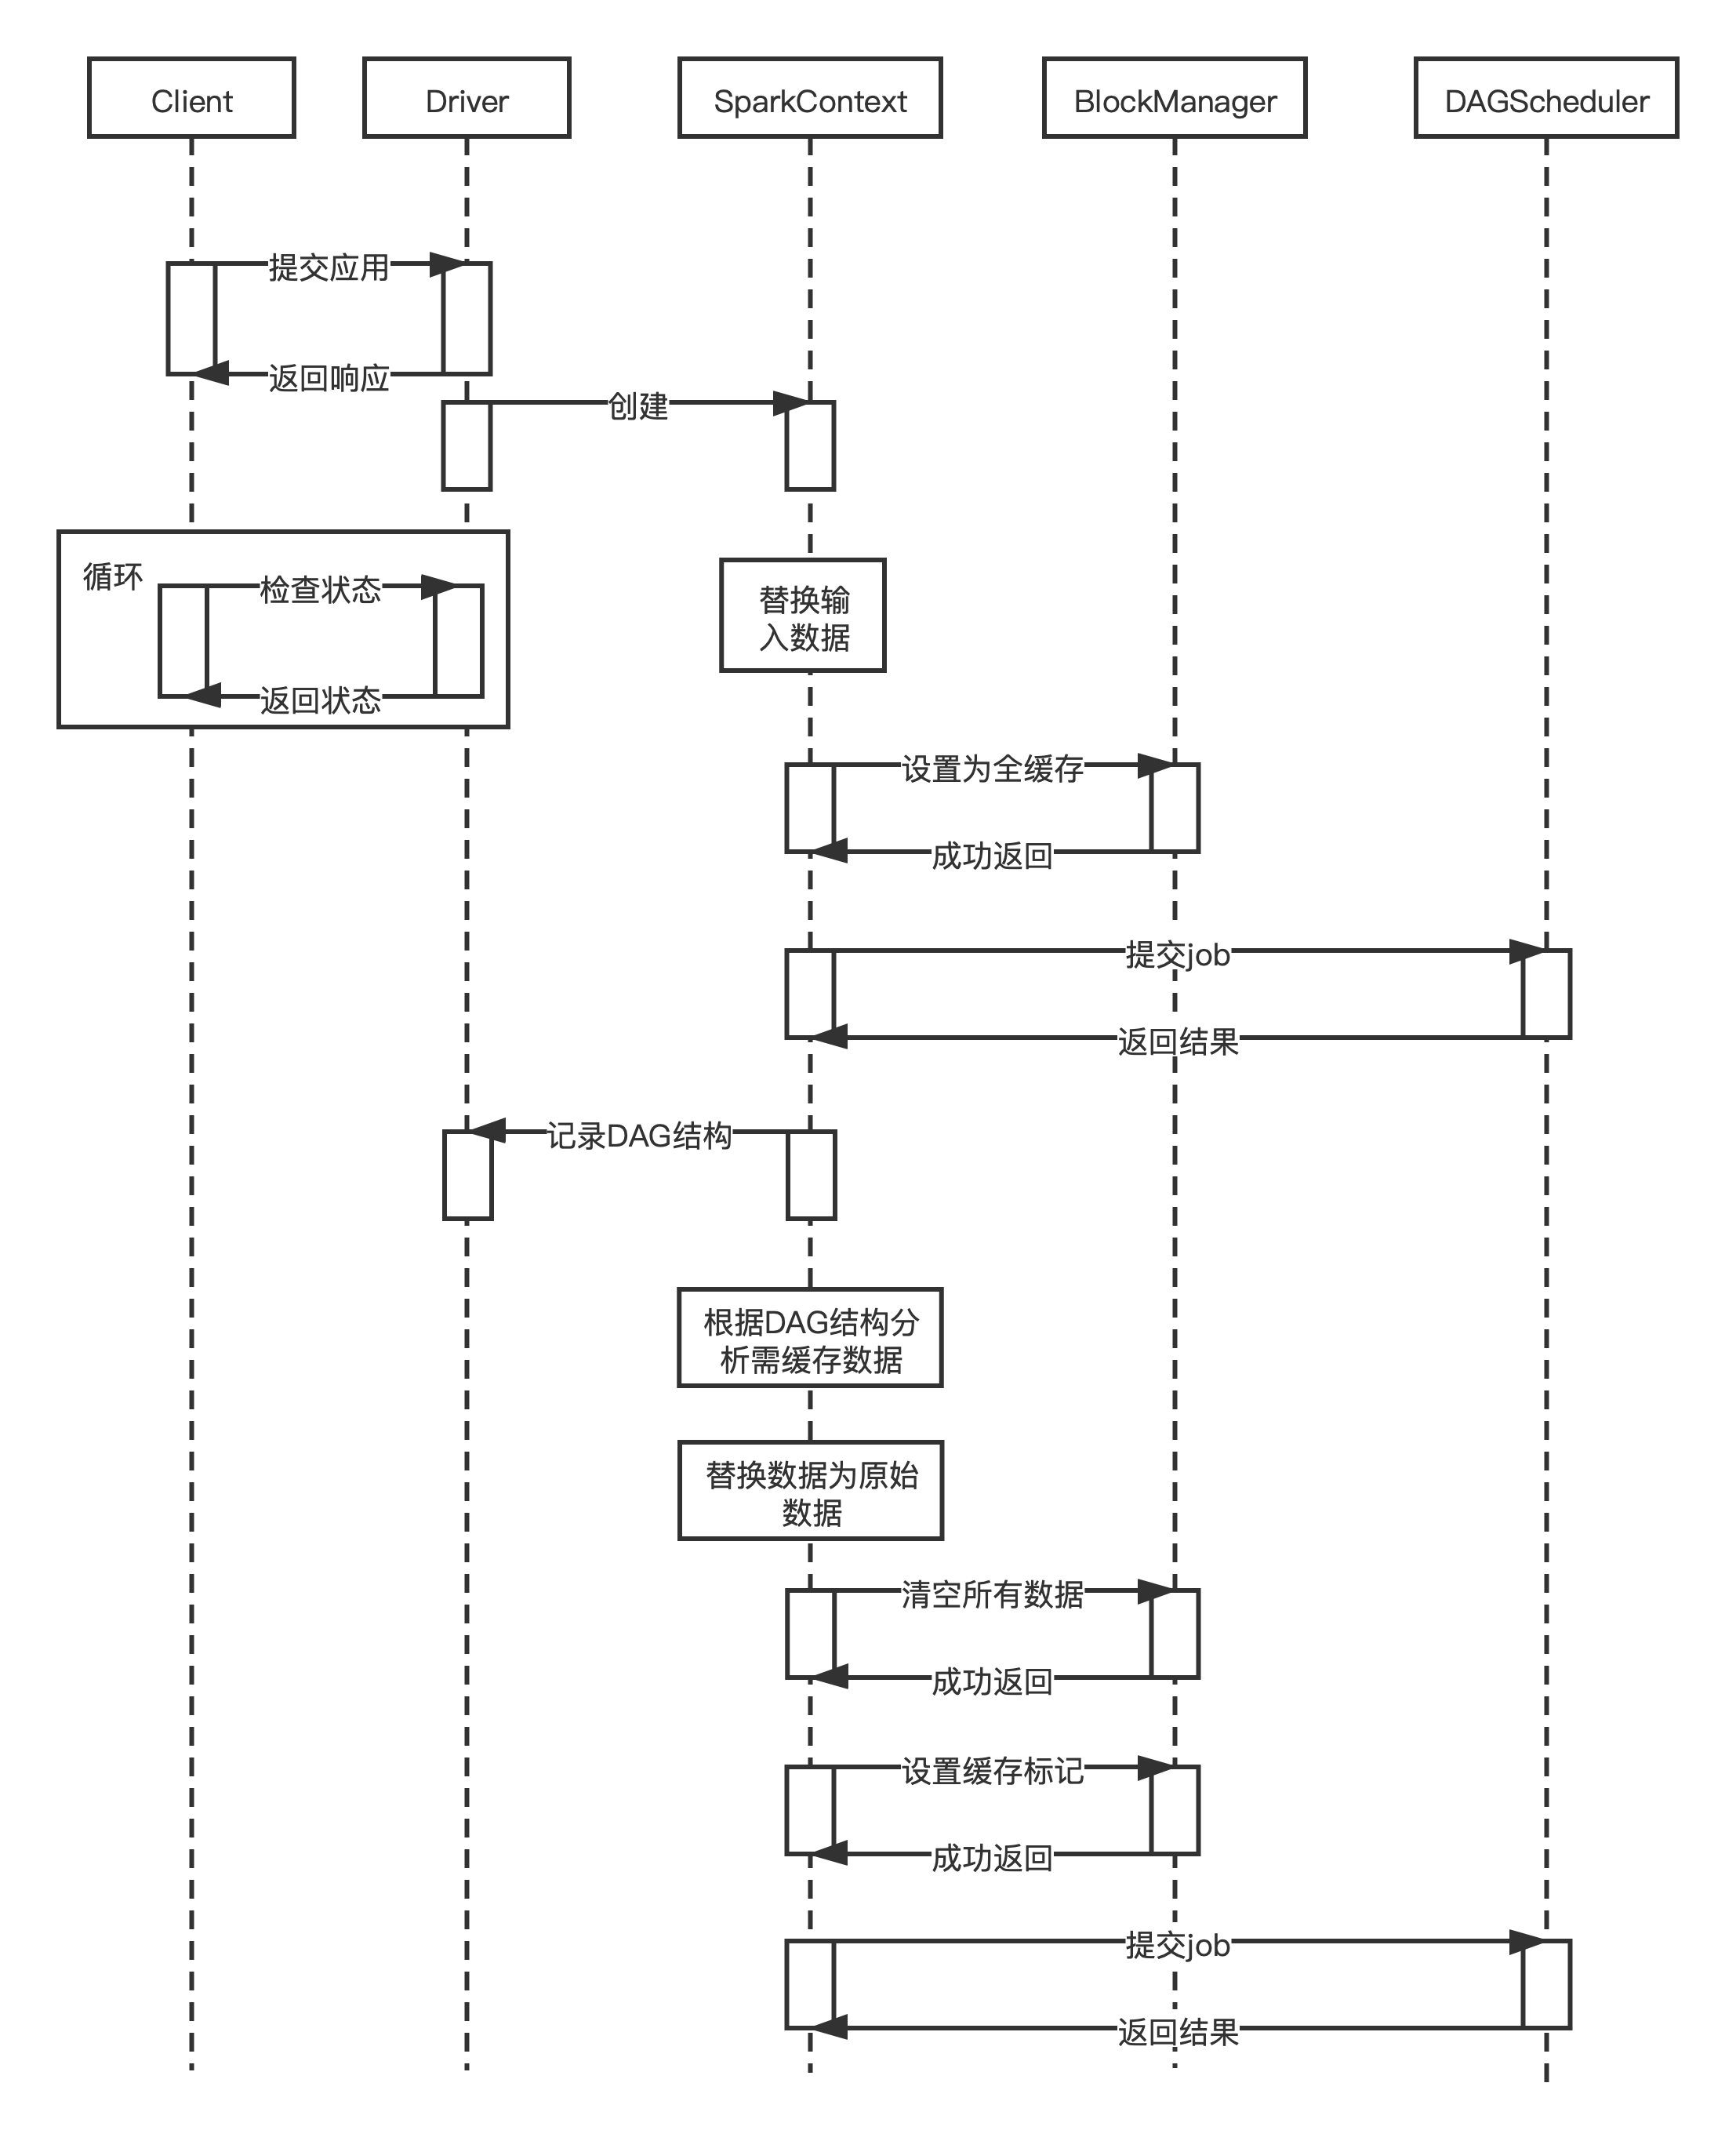
\includegraphics[width=1\textwidth]{Img/自动缓存流程图.png}
    \caption{自动缓存流程图}
    \label{fig:auto-cache}
\end{figure}

\begin{algorithm}  
    \caption{根据DAG图计算RDD使用频率}  
    \begin{algorithmic}[1] %每行显示行号  
        \Require DAG图根节点
        \Ensure 所有RDD使用频率
        \Function{CALCULATE\_FREQUENCY}{$RDD \ root, HashMap \ frequency$}  
            \State $id \gets root.getId()$
            \State $parent \gets root.getDependencies()$
            \For{$preRdd \in parent$}
                \State $preId \gets preRdd.getId()$
                \State $frequency[preId] \ frequency[preId] + 1$
                \State \Call{$CALCULATE\_FREQUENCY$}{$preRdd, \ frequency$}
            \EndFor
        \EndFunction  
    \end{algorithmic}
    \label{alg:cal-fre}
\end{algorithm}

\begin{algorithm}  
    \caption{清空缓存数据}  
    \begin{algorithmic}[1] %每行显示行号  
        \Require DAG图根节点
        \Function{CLEAN\_CACHE}{$RDD \ root$}  
            \State $root.unpersist()$
            \State $parent \gets root.getDependencies()$
            \For{$preRdd \in parent$}
                \State \Call{$CLEAN\_CACHE$}{$preRdd$}
            \EndFor
        \EndFunction
    \end{algorithmic}
    \label{alg:clean-cache}
\end{algorithm}


\begin{algorithm}  
    \caption{设置缓存标记}  
    \begin{algorithmic}[1] %每行显示行号  
        \Require DAG图根节点
        \Function{SET\_CACHE\_FLAG}{$RDD \ root, HashMap \ frequency$}
            \State $id \gets root.getId()$
            \State $rddFre \gets frequency[id]$
            \If{rddFre \ge 2}
                \State $root.STORAGE\_LEVEL \gets MEMORY\_ONLY$
            \EndIf
            \State $parent \gets root.getDependencies()$
            \For{$preRdd \in parent$}
                \State \Call{$SET\_CACHE\_FLAG$}{$preRdd, \ frequency$}
            \EndFor
        \EndFunction
    \end{algorithmic}
    \label{alg:set-cache}
\end{algorithm}

通过图\ref{fig:auto-cache}所示的流程,可以在第一次小规模计算结束之后得到整个DAG图的结构。然后通过算法\ref{alg:cal-fre}计算所有RDD节点的使用频率。得到频率之后便利整个DAG图,先调用unpersist接口清空小数据的缓存,再根据计算的到的频率设置各个RDD的STORAGE\_LEVEL之后修改输入节点的数据,替换为大规模数据,这样做有一下优点:

\begin{enumerate}
    \item 避免重复创建SparkContext对象,节约额外开销。在分析了自动缓存模块的实现原理之后可以发现因为需要通过运行整个应用获得DAG图,所以无法避免会带来一些额外开销。通过直接修改输入节点数据,就可以避免重复创建SparkContext对象,从而极大地减少了额外开销。
    \item 利用容错原理简化实现过程。通过流程图\ref{fig:auto-cache}可以设置rdd的缓存标记。设置完成之后只需要通过submitJob接口重新提交DAG图最后一个job即可。因为小规模数据缓存已经全部被清空,并且输入数据已经被替换,所以框架会根据基于血缘的容错原理从头开始执行整个DAG图。
\end{enumerate}

在第二次执行过程中,DAGScheduler会将job分为多个stage执行,在一个stage执行结束之后,会优化下一个stage的执行计划,此时根据调整自动缓存模块同步修改DAG图结构。实际上,目前自动执行框架只会做比较细粒度的执行计划,对DAG图整体结构并不会做出太大爱的调整。

\section{测试与性能分析}

为了测试自动缓存模块的效果,本文修改了Spark3.0的代码,实现了上述自动缓存模块的功能。然后通过SparkBench测试,下文也是使用SparkBench测试,本章简单的介绍以下SparkBench的功能和使用。

\subsection{SparkBench介绍}

SparkBench是Spark系统的基准性能测试项目,由IBM Watson研究中心的五名研究者发起,最后贡献给开源社区。SparkBench的测试项目覆盖了Spark最常见的四种应用:SQL查询、机器学习、图计算和流式计算。每种应用类型都选取了最常见的几个算法进行测试。SparkBench框架的测试结果包含系统资源消耗,计算时间,网络磁盘IO。所以可以比较全面地分析Spark系统的特点。官网也提供了论文。SparkBench支持表\ref{tab:workload}所示的负载。

\begin{table}
 \centering
 \caption{SparkBenck支持的负载}
 \label{tab:workload}
 \begin{tabular}{lcccl}
  \toprule
  应用类型 & 测试负载 \\
  \midrule
  机器学习 & 逻辑回归、支持向量机,矩阵分解  \\
  图计算 &  PageRank,SVD++,三角计数(Triangle Count) \\
  SQL查询 & Hive,RDDRelation  \\
  流式计算 & Twitter Tag , Page View  \\
  其他 &  Kmeans,线性回归,决策树,最短路径,标签传播,连通图,强连通图 \\
  \bottomrule
 \end{tabular}
\end{table}

SparkBench测试数据大部分都可以通过自带的数据生成器生成。SparkBench的使用也比较简单,分为以下三步:

\begin{enumerate}
    \item 修改<workload>/conf/env.sh文件,配置测试配置数据
    \item 使用<workload>/bin/gen\_data.shs生成测试数据,这个脚本会根据配置的数据生成指定大小的测试数据
    \item 调用<workload>/bin/run.sh运行测试负载
\end{enumerate}

测试样例运行完毕之后,测试数据会存放在num目录下面。包含作业运行过程中的资源使用情况,作业执行时间。资源使用情况包含CPU、内存的使用情况,磁盘和网络IO的使用情况。

\section{测试与分析}

本实验在一台PC电脑上实现,通过参数设置Spark为local mode,同时设置Spark为local模式运行。给Spark框架分配了8GB的内存。6个CPU。具体硬件配置与原件版本如表\ref{tab:setup}所示。

\begin{table}
 \centering
 \caption{测试环境硬件配置与软件版本}
 \label{tab:setup}
 \begin{tabular}{lcl}
  \toprule
  配置项 & 配置信息 \\
  \midrule
  CPU &  2.6GHz 6-core 9th\-generation Intel Core i7 processor \\
  内存 & 16GB of 2666MHz DDR4 memory  \\
  磁盘 &  512GB of SSD storage \\
  Spark版本 & 3.0.0  \\
  Hadoop版本 &  3.2 \\
  Scala版本 & 2.11.8  \\
  JDK版本 &  java\-1.8.0\_231 \\
  操作系统 & macOS 11 Big Sur  \\
  开发环境 &  IntelliJ IDEA 11.1.4 \\
  \bottomrule
 \end{tabular}
\end{table}

本文选用了逻辑回归、HIVE、PageRank、矩阵分解四个测试负载,在不同输入数据大小情况下,测试对比了自动缓存模块的效果。首先我对四个测试样例进行了测试,统计了Shuffle数据、Stage数量、Task数量等信息。通过测试可以发现不同的测试负载各有特点。比如对于逻辑回归类型应用,它并不存在shuffle操作,所以shuffle的读写数据都为0。对于HIVE应用,因为HIVE SQL查询最终生成的逻辑执行计划是一样的,又因为stage是根据宽依赖也就是shuffle依赖确定的,所以stage数量是相同的,但是因为数据量变大之后分区数量也随之变大,每一个分区对应一个task,所以随着数据量变大,task数量也会变多。对于PageRank算法,每次迭代后如果和上次的排名没有区别算法就认为已经收敛,然后推出结束了,数据规模比较小时收敛速度比较快,数据量大的情况下收敛速度变慢,迭代的轮数也会变多,导致stage数量也会变多。

\begin{table}
 \centering
 \caption{SparkBenck支持的负载}
 \label{tab:workload}
 \begin{tabular}{lccccccccccccccccl}
  \toprule
  负载名称 & 输入数据大小 & Shuffle 读/写 数据量 & Stage 数量 & Task 数量 \\
  \midrule
  逻辑回归 & 2G & 0G/0G & 3 & 431 \\  
  逻辑回归 & 4G & 0G/0G & 4 & 513 \\  
  逻辑回归 & 8G & 0G/0G & 5 & 1152 \\  
  逻辑回归 & 16G & 0G/0G & 7 & 2254 \\  
  HIVE & 2G & 2.7G/2.8G & 12 & 2927 \\  
  HIVE & 4G & 4.6G/4.8G & 12 & 6272 \\  
  HIVE & 8G & 10.3G/11.6G & 12 & 10048 \\  
  HIVE & 16G & 21.3G/22.7G & 12 & 20174 \\ 
  PageRank & 2G & 7.4G/9.4G & 6 & 1578 \\  
  PageRank & 4G & 15.4G/18.6G & 8 & 3481 \\  
  PageRank & 8G & 27.7G/31.8G & 13 & 5727 \\  
  PageRank & 16G & 62.3G/67.7G & 21 & 12247 \\
  矩阵分解 & 2G & 0.7G/0.9G & 9 & 394 \\  
  矩阵分解 & 4G & 1.2G/1.3G & 20 & 757 \\  
  矩阵分解 & 8G & 2.8G/3.1G & 43 & 1556 \\  
  矩阵分解 & 16G & 5.0G/5.4G & 81 & 4302\\  
  \bottomrule
 \end{tabular}
\end{table}

之后本文测试了自动缓存模块的效果,测试方法是修改了SparkBench测试负载的代码(在legacy分支),将代码中的cache调用全都删除,修改后运行添加了自动缓存模块的Spark框架。之后再与未修改的原生Spark框架进行对比。测试结果如图\ref{fig:auto-cache}所示。对于四个测试样例,一共进行了4组测试。每组测试分为两个样例,分别是手动缓存测试程序和自动缓存模块的对比。可见,自动缓存因为需要执行一遍得到整个DAG图结构,所以不可避免会导致一些额外的开销。使用自动缓存的模块实际运行时间变化不大。总体来说,因为使用自动缓存模块对于迭代式运算作业会带来12\%的额外开销,对于SQL类作业会带来3\%的额外开销。
\begin{figure}
    \centering
    \begin{subfigure}[b]{0.45\linewidth}
      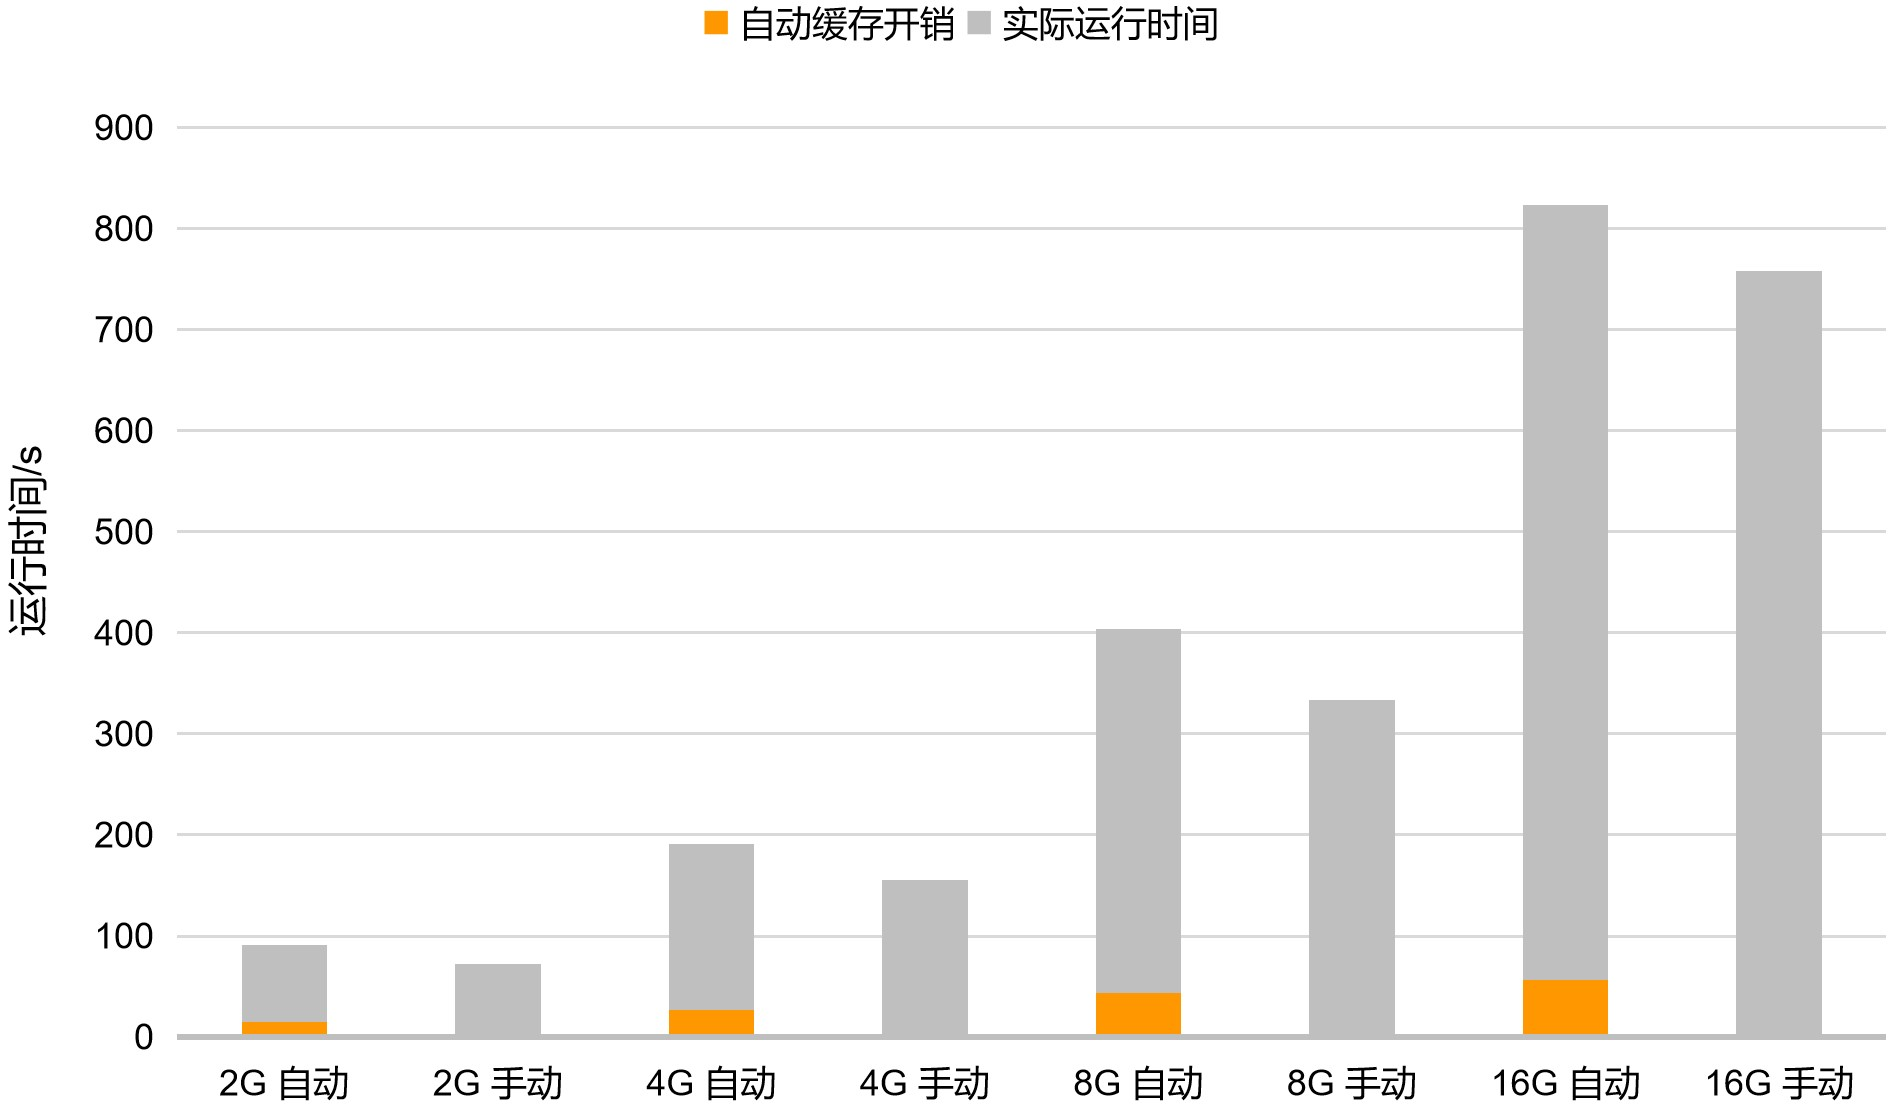
\includegraphics[width=\textwidth]{Img/lr1.jpg}
      \caption{逻辑回归测试}
      \label{fig:lr-auto-cache}
    \end{subfigure}%
    ~% add desired spacing
    \begin{subfigure}[b]{0.45\linewidth}
      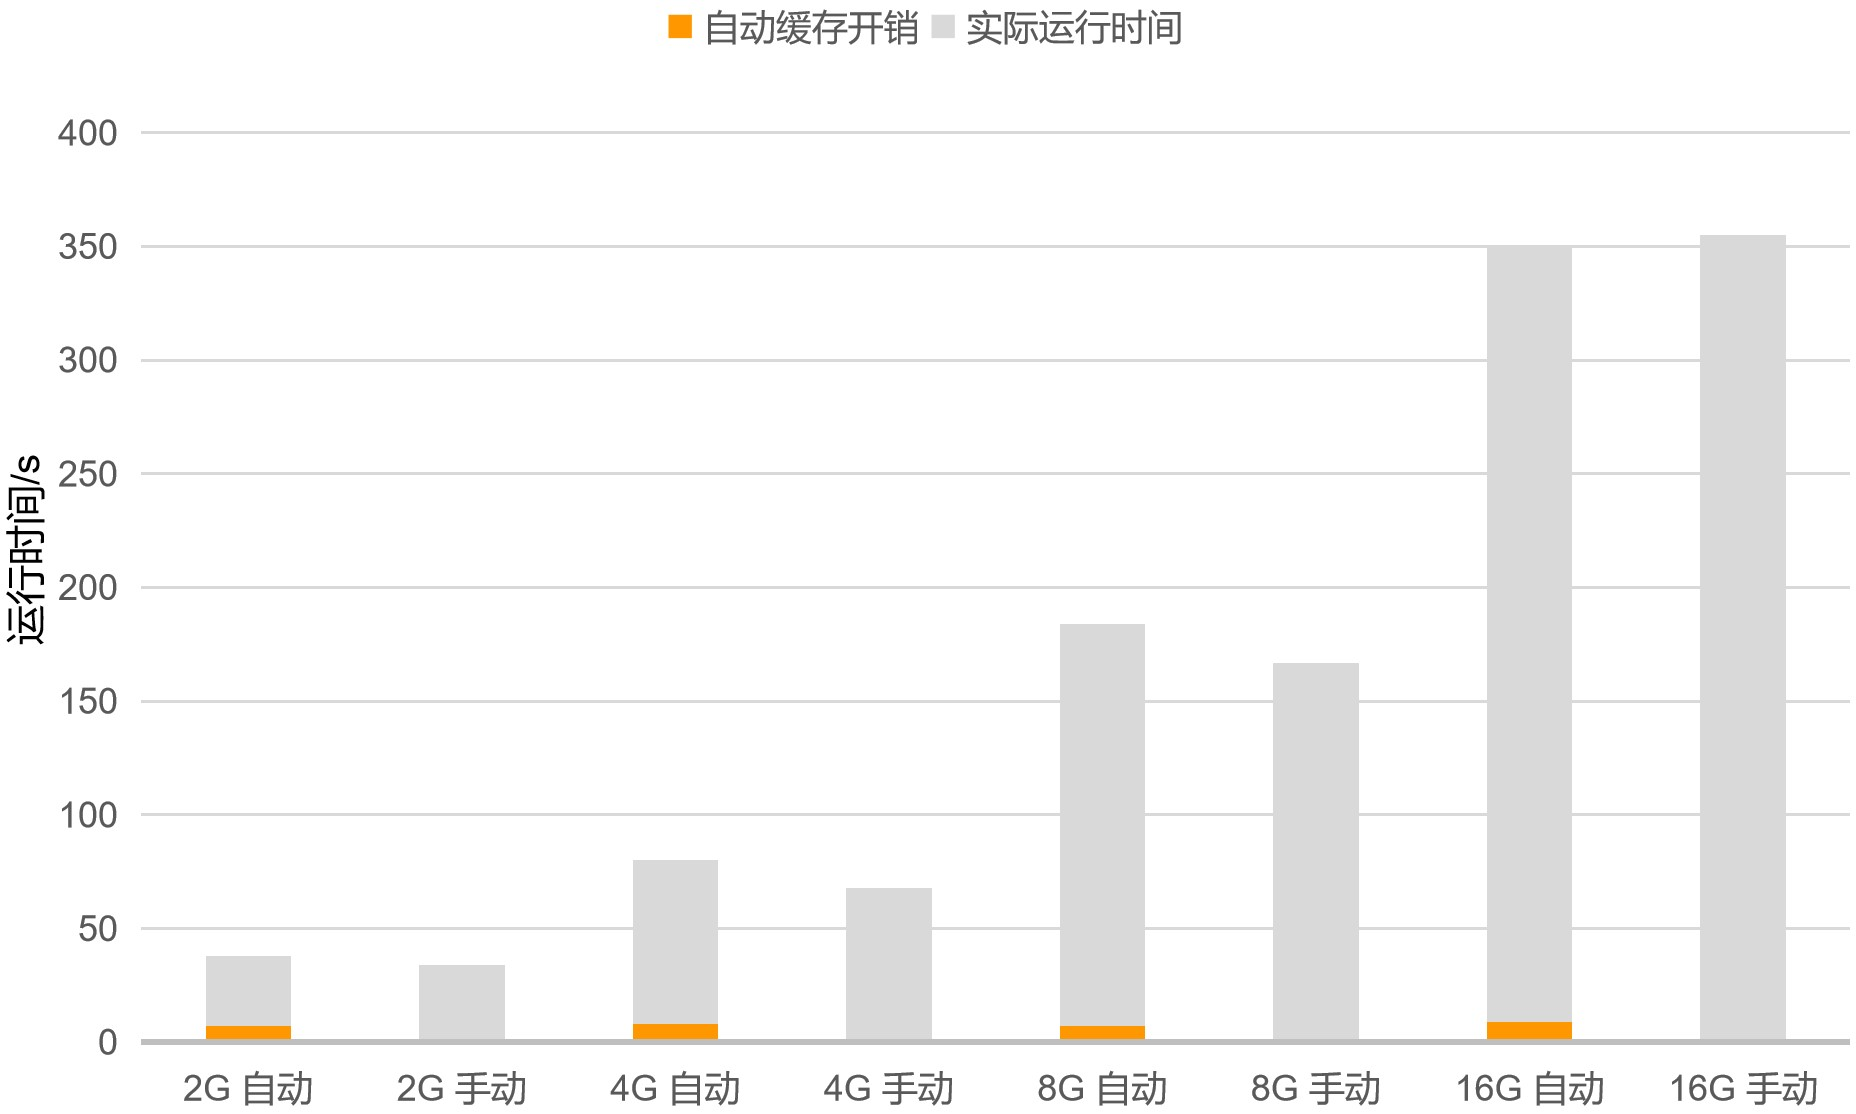
\includegraphics[width=\textwidth]{Img/hive1.jpg}
      \caption{HIVE SQL测试}
      \label{fig:hive-auto-cache}
    \end{subfigure}
    \\% line break
    \begin{subfigure}[b]{0.45\linewidth}
      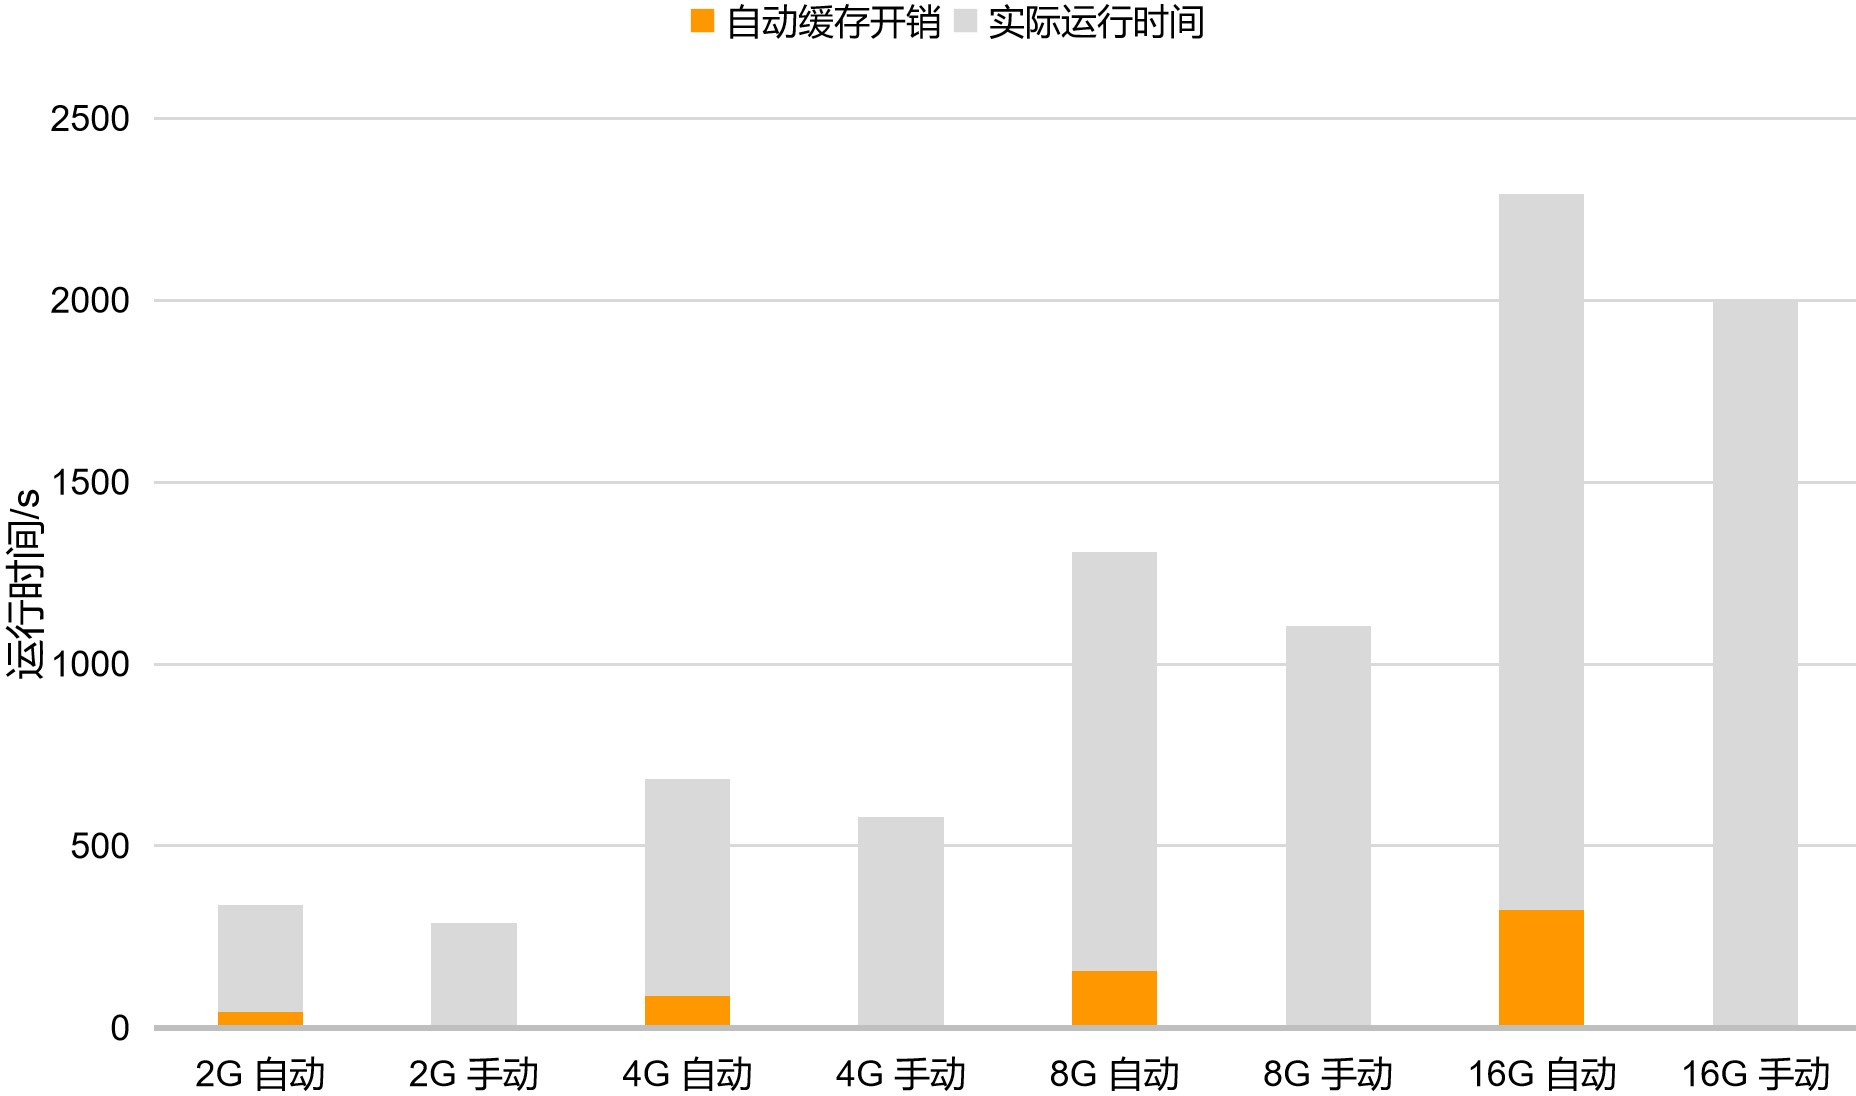
\includegraphics[width=\textwidth]{Img/pg1.jpg}
      \caption{PageRank测试}
      \label{fig:pagerank-auto-cache}
    \end{subfigure}%
    ~% add desired spacing
    \begin{subfigure}[b]{0.45\linewidth}
      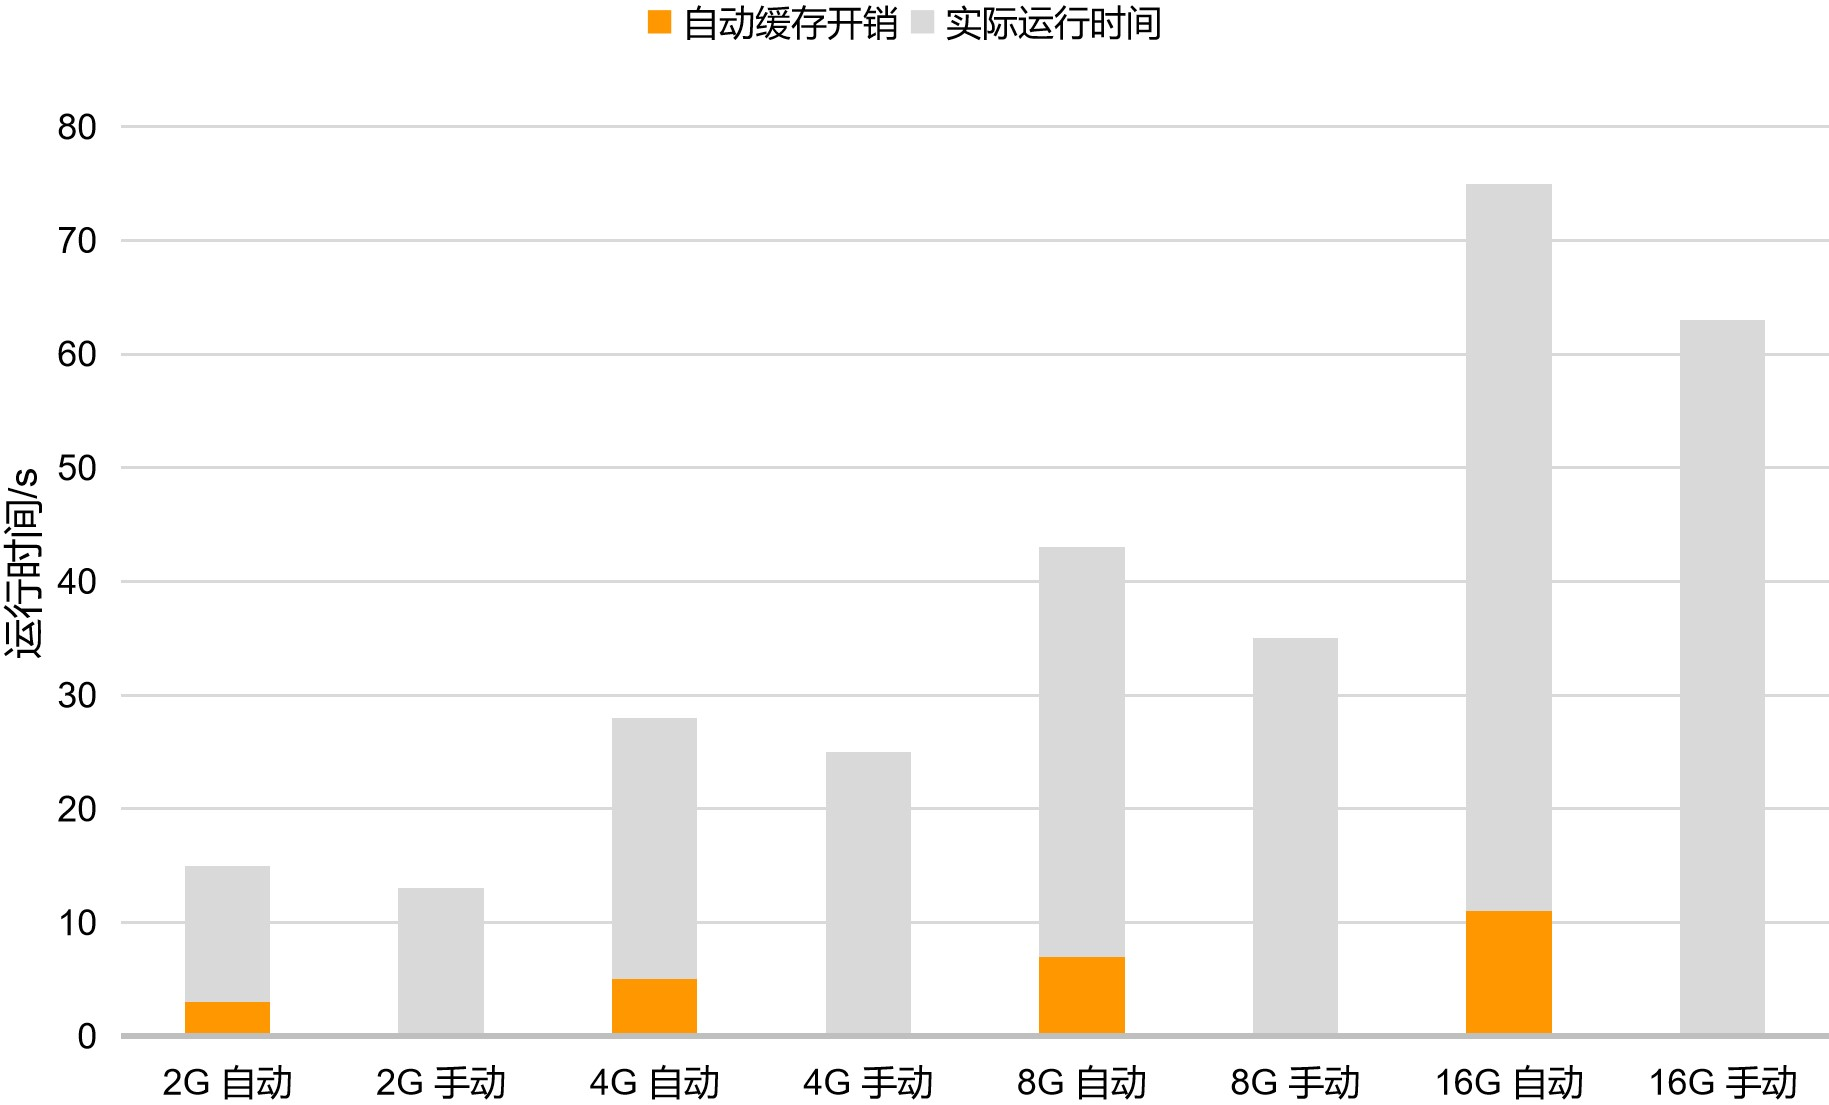
\includegraphics[width=\textwidth]{Img/mx1.jpg}
      \caption{矩阵分解测试}
      \label{fig:matrix-auto-cache}
    \end{subfigure}
    \caption{自动缓存测试}
    \label{fig:auto-cache}
\end{figure}

从图\ref{fig:autocache-2}可以看到,对于逻辑回归、PageRank和矩阵分解来说,额外开销会随着数据规模变大而变大,这与自动缓存和算法实现原理有关。因为这三种算法随着数据规模变大,迭代次数也会变多,所以第一次执行也需要迭代很多次才能得到DAG图结构,就会造成比较大的延迟。而对于HIVE SQL作业来说,随着数据规模变大额外开销并不会随之变化太多。这是因为对于SQL查询作业来说,在SQL转化得到的逻辑执行计划并不会随着输入数据变化,所以不同数据规模的自动缓存模块执行的逻辑执行计划都是一样的,就不会有太大的差别。

\begin{figure}
    \centering
    \begin{subfigure}[b]{0.45\linewidth}
      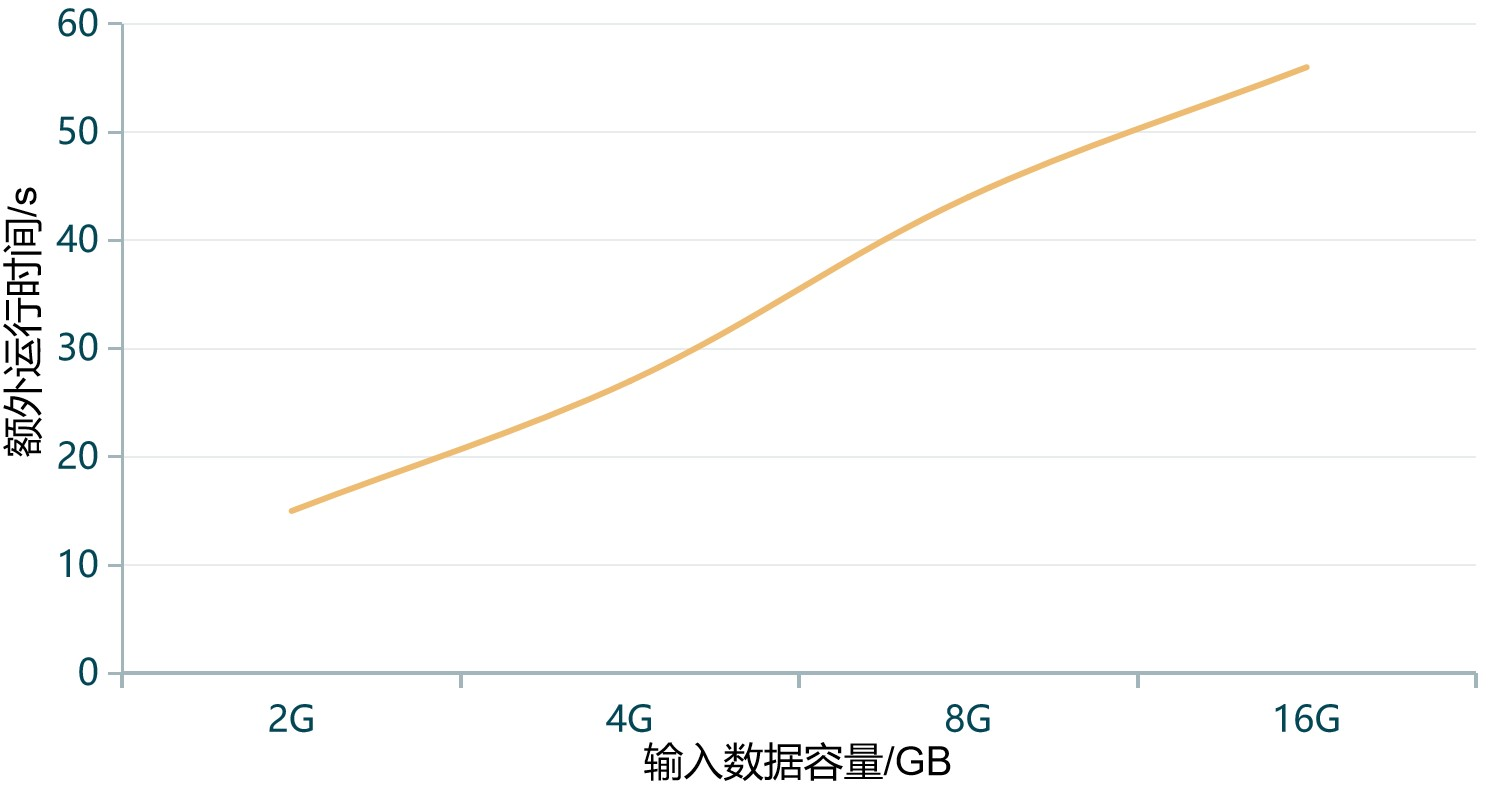
\includegraphics[width=\textwidth]{Img/lr2.jpg}
      \caption{逻辑回归测试}
      \label{fig:lr-ac-2}
    \end{subfigure}%
    ~% add desired spacing
    \begin{subfigure}[b]{0.45\linewidth}
      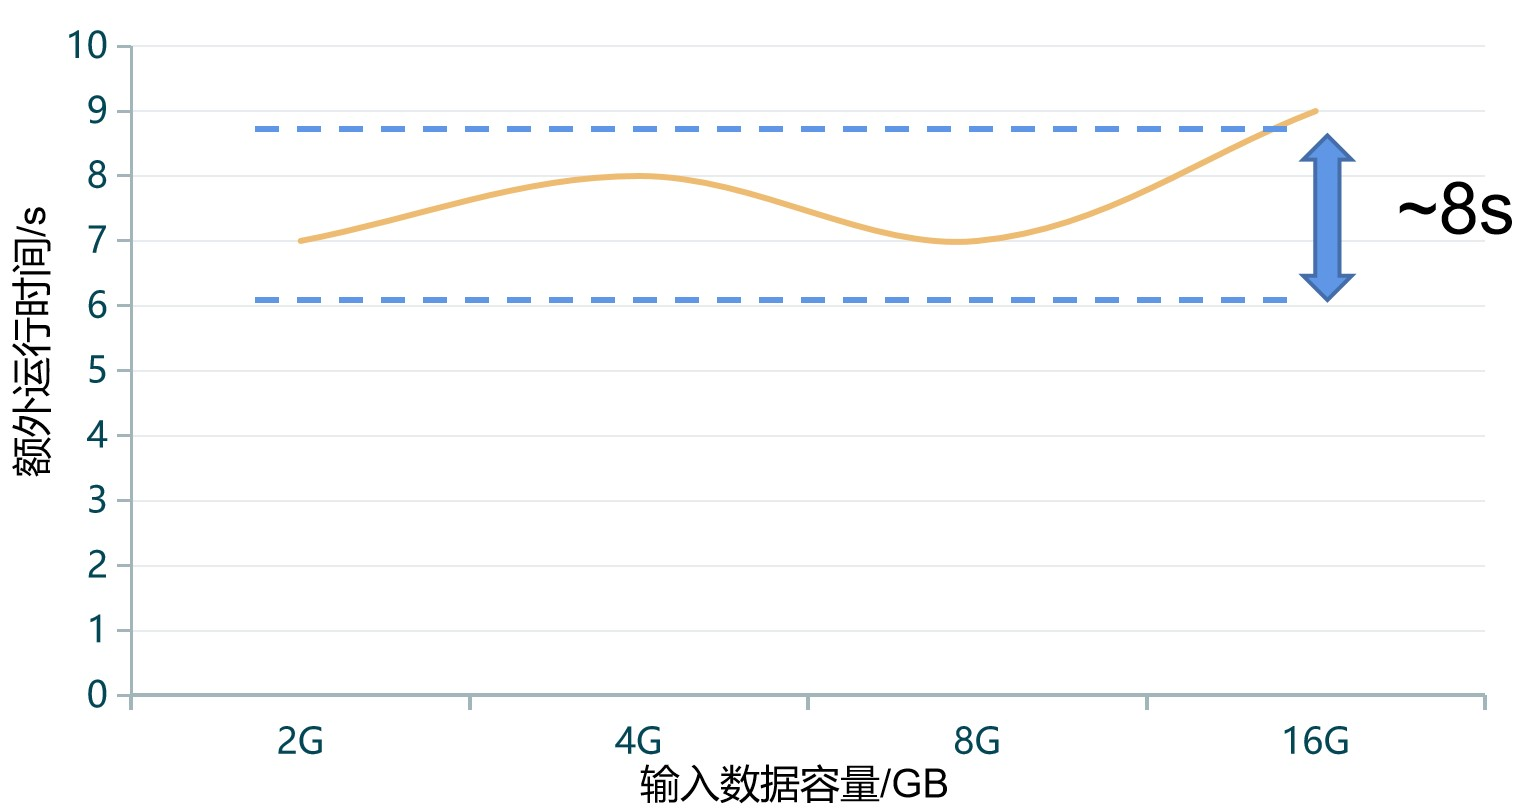
\includegraphics[width=\textwidth]{Img/hive2.jpg}
      \caption{HIVE SQL测试}
      \label{fig:hive-ac-2}
    \end{subfigure}
    \\% line break
    \begin{subfigure}[b]{0.45\linewidth}
      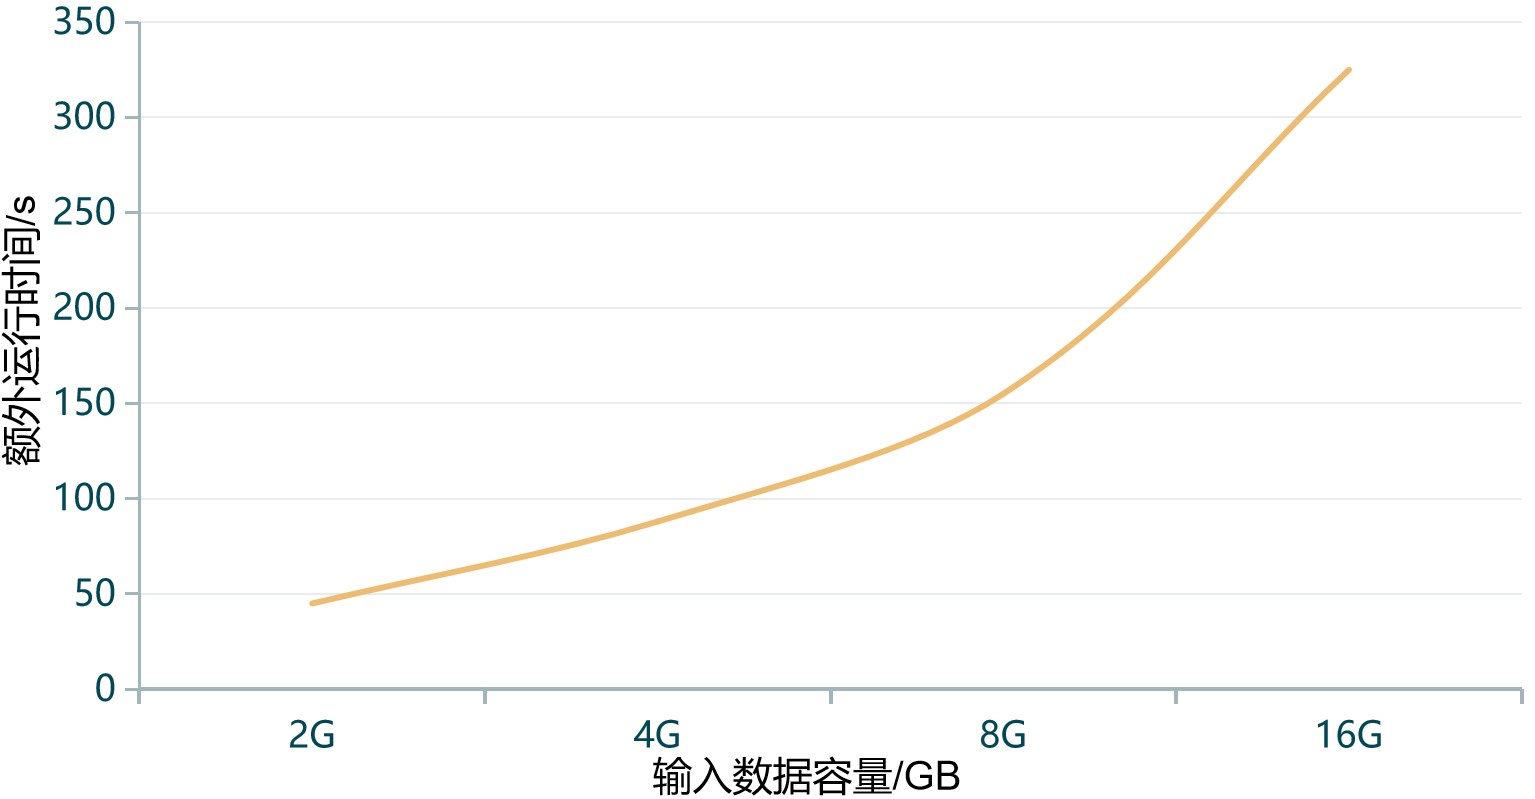
\includegraphics[width=\textwidth]{Img/pg2.jpg}
      \caption{PageRank测试}
      \label{fig:pagerank-ac-2}
    \end{subfigure}%
    ~% add desired spacing
    \begin{subfigure}[b]{0.45\linewidth}
      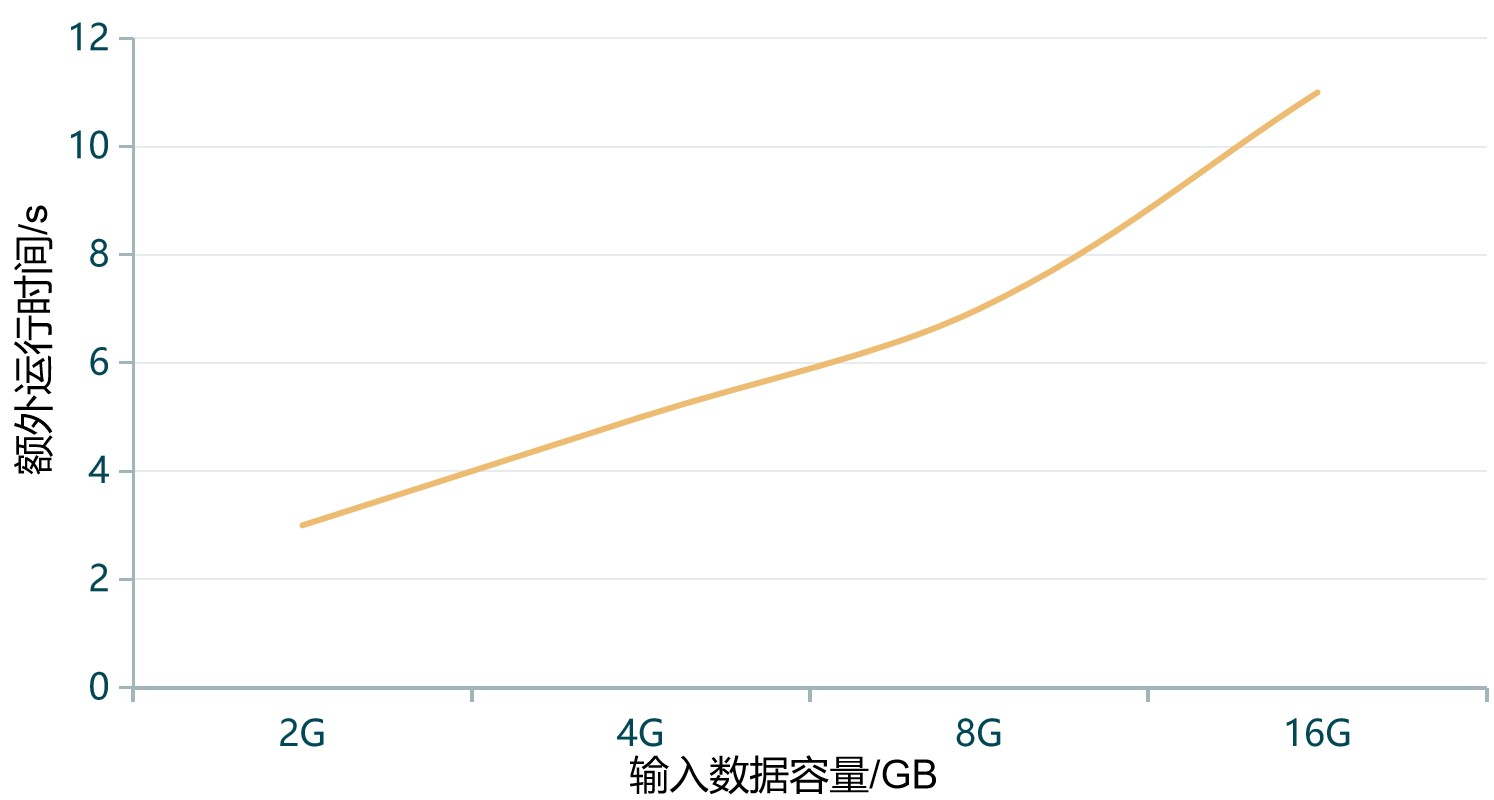
\includegraphics[width=\textwidth]{Img/mx2.jpg}
      \caption{矩阵分解测试}
      \label{fig:matrix-ac-2}
    \end{subfigure}
    \caption{自动缓存额外开销测试}
    \label{fig:autocache-2}
\end{figure}

总结可以总结以下结论,自动缓存模块对于SQL作业效果比较好,随着数据规模变大,额外开销占比越来越小。而对与PageRank这类迭代式计算应用则效果一般,因为这类应用随着数据规模变大,迭代次数也会变大,额外开销也会随着迭代次数变多而随之变大。

\section{本章总结}

本章介绍了Spark模块底层的原理以及最新的Spark自适应执行特性。之后设计并实现了自动缓存模块,自动缓存模块通过分析DAG图结构得到需要缓存的数据并自动将其缓存到内存之中。最后对自动缓存模块进行了一系列的测试,实验测试结果表明自动缓存模块适合SQL查询类作业,因为这类作业不同数据规模的执行计划相同,所以数据规模越大自动缓存模块额外开销占应用运行总时间越短。但是不太适合迭代计算式作业,因为大规模数据迭代次数变多额外开销也会随之变大。最后经过计算,对于迭代式计算和SQL作业,自动缓存模块平均额外计算开销占作业总执行时间的12\%和3\%。

